%----------------------------------------------------------------------------
\chapter{\AudioOverIp}
%----------------------------------------------------------------------------
\section{Bevezetés az Audio over IP világába~\cite{AHNERT2023}}
%----------------------------------------------------------------------------
A 90-es évek vége óta a szakmai hangipar elmozdult a pont-pont digitális
átviteli formátumoktól mint az AES/EBU vagy a MADI az IP-alapú szabványok felé a példa kedvéért mint az AES67. 
Ez a csomag alapú hálózati megközelítés hatalmas rugalmasságot
hozott, valamint kibővített vezérlési és monitorozási képességeket biztosít a
hangmérnökök számára. Lehetőséget kapunk arra, hogy egy fizikailag már meglévő
telepítést későbbi szoftverkonfigurációval és frissítésekkel bővíthetővé tegyünk.
A gyártók különböző esetekben akár teljesen új funkciókkal is kiegészíthetik a már meglévő eszközöket,
habár ez elsősorban csak a prémium kategóriás eszközökre igaz.

A jelutak az IP alapú gondolkodásmód miatt már nem kötődnek 1:1 fizikai kábelekhez, hanem
bármikor pár egérkattintással megváltoztathatóak anélkül, hogy szükség lenne bármilyen
jellegű fizikai átrendezésre, vagy dedikált audio útválasztó hardverre. 
A csomagorientált átvitel jellegéből adódik, hogy az audiojelek automatikusan eljutnak 
a kívánt helyre a hálózaton keresztül.

A Cirrus Logic által 1996-ban bevezetett CobraNetet
tekintik általában az első sikeres audio-over-ethernet hálózat-implementációnak.
Bár még ma is sok CobraNet telepítés létezik, magas késleltetési problémák és korlátozott skálázhatóság
miatt nem ideális élő hang, stúdiók és rádióállomások számára.

A mintegy tíz évvel később megjelent egy ausztrál cég az Audinate, és az általuk kifejlesztett
Dante a `Digital Audio Network Through Ethernet'. Dante sok jelentős
előnnyel rendelkezik az első generációs audio-over-IP technológiákhoz viszonyítva.
Ezek közé értve a jobb használhatóságot és magasabb kompatibilitást a szabványos
IT infrastruktúrával. A Dante egy hatalmas hardveres ökoszisztémából is profitál, 
több száz gyártó által gyártott ezernél is több eszközzel szerte a világon.

Mielőtt a Dante elérte volna jelenlegi domináns pozícióját, nagy várakozás volt az AVB
(Audio Video Bridging) nevű technológia körül is.
Az autóipar és az ipari automatizálás, átvette az AVB-t, és
általánosabb nevet adtak neki, mivel már nem csak hang és videóalkalmazásokhoz kapcsolódott
Az AVB-t a gyártók fejlesztőcsoportja, AVnu Alliance időérzékeny hálózat (TSN) néven nevezte el.

Később a Milan munkacsoport, ami egy audio/video gyártókból álló konzorcium, úgy
döntött, hogy kidolgoz egy finomhangolt specifikációt a profi audio/video
rendszerekben való használatra, Milan néven.
Ez egy specifikus TSN verzió, amely az audio/video szolgáltatók közötti interoperabilitásra összpontosít.
Fontos, hogy nem a TSN alapján készült, mivel a TSN-hez speciális IT hardver szükséges az audio
követelmények kezeléséhez, és csak korlátozott számú kapcsoló támogatja a TSN-t.

Az átmenet az IP hálózatokra összehasonlítható az analóg hangról a digitális
hangra való átmenettel. Először csak néhány kezdeti telepítés, amelyek az új technológiát
használják, majd esetleg hiányosságokat mutathatnak a kezelés vagy a megbízhatóság
terén a hagyományos régi megközelítéshez képest, de ezek idővel a technológia fejlődésével eltűnnek. 

Vannak területek, ahol az IT hálózatok alapvetően más módon működnek, mint a hagyományos audio útválasztás.
Először is, egy szabványos IT hálózat nem arra van kialakítva, hogy szigorú időzítési követelményeket kelljen teljesítenie, 
azonban ez általában az audio esetében nagyon is szükséges.
Egy hálózati környezetben az adatcsomagok útját más csomagok is akadályozhatják, ami jelentős
időbeli változást eredményezhet az csomagok érkezési idejénben.
A hagyományos audio kábelek esetében az adatok továbbításának időzítése nem változott meg a kábel által.
Egyig végponttól a másikig a hangminták zavar nélkül (feltételezve, hogy a kábel jó minőségű és nincsen interferencia) 
érkeznek meg. Az IT hálózatokban azonban a csomagok útja nem garantált, és a csomagok késleltetése változhat.
Másodszor, egy csomag elvesztése elfogadhatónak tűnhet és tűnik is egy szokásos IT
alkalmazás esetében, mivel azok automatikusan újraküldésre kerülnek, amennyiben valami hiba során elvesznek.
Az audio alkalmazások esetében a késleltetés minimalizálása érdekében
létfontosságú, hogy a csomagok az első alkalommal a korrekt helyre érkezzenek meg, mivel egyáltalán nincs semennyi
idő sem az újraküldéshez. Ha néhány csomag elveszik, az azonnal hallható megszakításokat és kimaradásokat okoz,
rongálva ezzel a hang élvezhetőségét.

A csomagvesztés gyakori okai a linkek túlterhelése, vagy a túl alacsony pufferméret.
Tehát az audiohálózatokat oly módon kell kialakítani, hogy elegendő sávszélesség álljon rendelkezésre
minden egyes eszköz számára egyidejű használat esetén is. 
Ha ez teljesül, és a csomagkiszállítás időben történik, ahogyan az audio alkalmazások igénylik,
akkor a hálózatunk már elméletileg képes lehet hosszútávon stabilan működni.
Ettől függetlenül érdemes túlbiztosítani a hálózatot oly mértékben, hogy minden csomag időben
megérkezzen, anélkül, hogy további extrém finomításra lenne szükség a kapcsolók
konfigurációjában. Konkrétan ez azt jelenti, hogy olyan IT hálózatokat kell
építeni melyek elegendő sávszélességgel rendelkeznek, és kizárólag az audio alkalmazások számára
legyen használatos, tehát ne keveredjenek általános mindennapi alkalmazásokkal.

A legtöbb audio-over-IP technológia abból indul ki, hogy az alapul szolgáló
hálózat megfelelően fog működni, hibamentesen végzi a dolgát. Gondolva itt arra, hogy nincsen csomagvesztés, 
nincs súlyos ütközés más csomagokkal a kapcsoló hardveren, és a csomagok nem késnek a hálózaton.
Néhány esetben, különösen ha az audio és más forgalmat keverik, 
fontos lehet az audio és szinkronizációs csomagoknak elsőbbséget biztosítani másokkal szemben,
például az internetes böngészéssel szemben. Ez a mai legtöbb kereskedelmi forgalmazott
kapcsolóval elérhető. \newline

Példa audio over IP hálózatokra:
%----------------------------------------------------------------------------
\begin{itemize}
	\item Audinate által kifejlesztett - Dante
\end{itemize}
\begin{itemize}
	\item QSC által kifejlesztett - Q-LAN
\end{itemize}
\begin{itemize}
	\item Lawo és Partnerei által kifejlesztett - RAVENNA
\end{itemize}
%----------------------------------------------------------------------------
\begin{figure}[H]
	\centering
	
\includegraphics[width=50mm, keepaspectratio]{figures/dante_logo.jpg}
	\caption{Audinate Dante logó}
	\label {fig:dante_logo}
\end{figure}
%----------------------------------------------------------------------------
\subsection{Előnyök és hátrányok}
%----------------------------------------------------------------------------
Az IT hálózatok alkalmazása hangkapcsolatokra nézve számos előnyt kínál:
\begin{itemize}
	\item Rugalmasság hangkapcsolatok hozzáadásához vagy módosításához anélkül,
	      hogy kábeleket cserélnénk.
\end{itemize}
\begin{itemize}
	\item Az IT viszonylag alacsony áron széles skálájú funkciókat kínál.
\end{itemize}
\begin{itemize}
	\item Alkalmazkodás és integráció az IT hálózati infrastruktúrákba
	      specifikus audio vagy videokábelek alkalmazása nélkül.
\end{itemize}
\begin{itemize}
	\item Videójel és vezérlési adatok továbbíthatók ugyanazon infrastruktúrán
	      keresztül.
\end{itemize}
%----------------------------------------------------------------------------
Ugyanakkor az audio-over-IP hálózatok felhasználóit számos kihívás elé is állíthatják:
%----------------------------------------------------------------------------
\begin{itemize}
	\item Azért mert általában több hangmintát egy csatornából egy csomagba helyeznek
	      el a hatékonyság érdekében, adott minimális késleltetés adódik, mivel az
	      küldőnek meg kell várnia, hogy a hangminták rendelkezésre álljanak, mielőtt
	      azokat átküldené a hálózaton. Ez a késleltetés általában magasabb, mint a
	      pont-pont digitális hangszabványok esetében, de optimalizált csomagformátumok és
	      hálózati beállítások segítségével minimalizálható és nagyon jól közelíthető.
\end{itemize}
\begin{itemize}
	\item Mivel az IT hálózatok nem meghatározottak a csomagok úti idejét tekintve,
	      egy biztonsági tartományt, azaz egy audio buffer-t kell beszúrni a fogadó végén.
	      Ez a buffer további késleltetést eredményez. Minél kevesebb csomagütközés van
	      jelen a hálózatban, annál inkább csökkenthető ez a biztonsági tartomány és
	      ezzel a késleltetés.
\end{itemize}
\begin{itemize}
	\item Az audio csomagformátumok változatossága miatt növekszik a komplexitás,
	      ami azt jelenti, hogy a fogadóknak és küldőknek azonos beállításokkal kell
	      rendelkezniük. Az audio-over-IP technológia komplexitása jelentősen magasabb,
	      mint az előző technológiáké. Az iparág még mindig jelentős munkát végez annak
	      érdekében, hogy csökkentse ezt a komplexitást a felhasználók számára, bevezetve
	      intelligens és felhasználóbarát szoftvermegoldásokat az audiohálózatok
	      kezelésére.
\end{itemize}
%----------------------------------------------------------------------------
\subsection{Fázishelyesség}
%----------------------------------------------------------------------------
A legtöbb audio alkalmazásban kritikus számunkra több eszköz szimultán szinkronizált viselkedése.
Elengedhetetlen az egyes mikrofonok vagy hangszórók közötti fázispontosság.
Amikor több hangszóró van csatlakoztatva egy erősítőhöz, és az összes csatorna
egyetlen hangcsomagban érkezik meg, nincs veszélye annak, hogy a csatornák
ellenfázisban lennének egymással, mivel a hangminták nem változhatnak el egymás
között a hálózaton keresztüli átvitel során. 

Azonban egy nagy rendszernél több erősítő és processzor függetlenül egymástól kap hangcsomagokat, 
az is lehetséges, hogy fizikailag is távolabb vannak egymástól,
miközben továbbra is szükség van arra, hogy pontosan reprodukálják a jeleket egyező fázissal.
Egy adott csomagot több hálózati eszköz is megkapja, puffereli, és ezeket
pontosan ugyanabban az időben kell lejátszaniuk.

Mivel nincsenek szoros időzítési specifikációk az IT hálózatokban a csomagok továbbításának és
megérkezésének időpontjára vonatkozóan, az audiohálózatoknak mindenképpen egy olyan szinkronizációs
módszert kell biztosítani ami megoldja számunkra ezt a rendkívül kritikus problémát.
Ez egy fontos, és egyben új probléma a audio hálózatokban, amellyel az összes
audio-over-IP technológiának foglalkoznia kell, nem lehet megkerülni.

Az audiohálózaton belül minden eszköznek abszolút időben szinkronizáltnak kell lennie
a Precision Time Protocol (PTP) szerint. Ez azt jelenti, hogy belső óráik (PTP
követők) egy referenciaóra eszközből (PTP vezető) származnak. Ez az eszköz
bármilyen audioeszköz lehet, amely biztosítja ezt a funkciót, vagy akár egy
speciálisan erre a célra fejlesztett eszköz is lehet a pontos PTP órák előállítására.
A vezetőt egy felhasználói beállítás vagy alternatívaként egy szabványos
automatizmus választja ki. Az összes eszköz számára, legyen az audio adó vagy
vevő, az a végső követelmény, hogy pontosan szinkronizálódjanak ehhez az adott időhöz.
Az audio csomagokat küldési pillanatukban egy időbélyegzővel látják el. A felhasználó állandó időeltolást állít be az
összes vevőnél, ez a linkeltolás. Amikor tehát a csomag megérkezik egy vevőhöz, a
pufferben marad, míg lejátszásra nem kerül. Tehát az audio lejátszás pillanata a
küldési idő plusz a linkeltolás. \newline

Minden vevő két feltétel mellett érheti el egymás között a fázispontosságot:
%----------------------------------------------------------------------------
\begin{itemize}
	\item Pontos időszinkronizálás a PTP óra vezetőjéhez (azonos időbázis).
	\item Azonos linkeltolási érték beállítása a felhasználó által az összes vevőeszközön.
\end{itemize}
%----------------------------------------------------------------------------
Ezért a linkeltolást az érintett összes kapcsolat legrosszabb esetű késleltetése alapján kell kiválasztani. 
Javasolt bizonyos engedményt hozzáadni az esetleges csomagkiszállítási idők váratlan eltéréseinek esetére.
Ez azt jelenti, hogy kicsivel nagyobb időt hagyunk az átlagos csomagfeldolgozási időnél, 
ezzel is biztosítva a rendelleneségektől mentes működést.
Szerencsére ez a koncepció elterjedt és jelenleg minden audiohálózati szabványban használatos. 
%----------------------------------------------------------------------------
\begin{figure}[H]
	\centering
	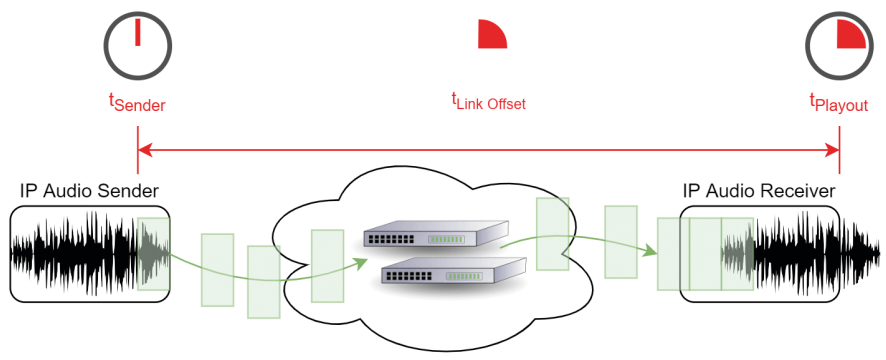
\includegraphics[width=\linewidth, keepaspectratio]{figures/link_offset_latency.png}
	\caption{A kapcsolati eltolás meghatározza a késleltetést~\cite{AHNERT2023}}
	\label {fig:link_offset_latency}
\end{figure}
%----------------------------------------------------------------------------
\begin{figure}[H]
	\centering
	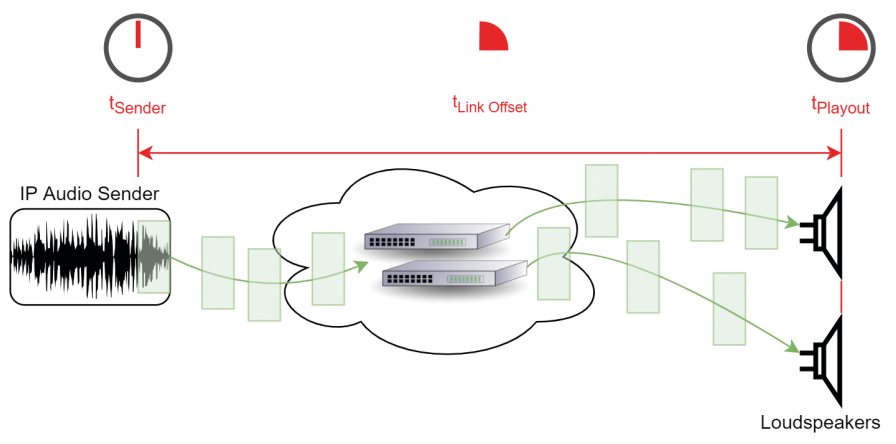
\includegraphics[width=\linewidth, keepaspectratio]{figures/phase_coherence_link_offset.png}
	\caption{Fáziskoherencia azonos kapcsolati eltolással~\cite{AHNERT2023}}
	\label {fig:phase_coherence_link_offset}
\end{figure}
%----------------------------------------------------------------------------
\subsection{Szinkronizáció}
%----------------------------------------------------------------------------
Az IP küldők és fogadók szinkronizációja az alacsony késleltetéssel való szinkronban lévő működéshez elengedhetetlen.
A hagyományos audio technológiákban az eszközöket vagy külön \textit{word clock} kapcsolattal, 
vagy szinkronizált audio formátumokkal, például AES/EBU vagy MADI segítségével szinkronizálták.

A fogadók közvetlenül képesek frekvenciájukat és fázisukat kinyerni,
mivel valamiféle \textit{impulzust} biztosítottak, ami jelzi a pillanatot, amikor egy
audio minta létrejön vagy lejátszódik, például analóg-digitális konverterek esetében is.
Az PTP csomagok kicsik és nem tartják fel a forgalmat sokáig, de fontos, hogy a
kapcsolókban a lehető legmagasabb prioritással továbbítsuk őket. 
Ez végül növelni fogja a szinkronizáció pontosságát, így a késleltetési eltérések minimalizálódnak.

A QoS (Quality of service) keretein belül a PTP csomagokat még a hangnál is magasabb prioritással kell
kezelni. Az összes hálózati eszköz ugyanazon naptári időpontra szinkronizálódik a Precision Time Protocol
(PTP) segítségével. Ennek az időnek a vezérlője egy olyan eszköz, amelyet óraleadernek
neveznek, míg az ehhez igazodó eszközöket óra követőknek hívják. 

Minden eszköznek meg le kell hozzá generálnia a hagyományos helyi órát is, amelyet a PTP-n keresztül kapott
abszolút időből származtat. Ez a belső óra a \textit{médiaóra}. 
Ha a gyártó megfelelően implementálja, minden eszköz médiaórájának pontosan ugyan annyinak kell lennie a
frekvencia és fázis terén. A magas pontosság technikailag elérhető, de kihívást
jelent a gyártók számára. Ezért a PTP szinkronizált eszközök közötti
fázispontosság minőségtől és árkategóriától függően változhat. Elfogadható változásnak tekinthető ha az
eltérés kisebb mint <1 µs, azaz 1 mikroszekundum.

Mivel az IT hálózatok nem eléggé determinisztikusak a csomag kézbesítésének időpontját
illetően, a készülékek pontos szinkronizációja kifinomult megközelítést igényel.
A PTP követők fő feladata két hatás kompenzálása, amelyek bármilyen hálózat esetén előfordulhatnak:
%----------------------------------------------------------------------------
\subsubsection{Jitter kompenzáció}
%----------------------------------------------------------------------------
A PTP vezető által a szinkronizációs üzenetekben megadott jelenlegi időt az összes követőnek egy jól ismert multicast
cím (224.0.1.129) használatával mutatják be. 
A hálózat és a kapcsolók természetéből adódóan ez az információ nem mindig érkezik meg tökéletes állandó
késleltetéssel a vevő számára. 
Ez a változás a csomag jitter vagy csomag késleltetési változás (PDV) néven ismert effektus,
ezt az elváltozást minden PTP követőnek kompenzálnia kell. 
Általában az audio hálózatok 1--8 üzenet/mp szinkronizálási arányt
használnak. A 8-as maximális érték csak kompatibilitás érdekében javasolt, egy ilyen
magas szinkronizálási arány nem szükséges a legtöbb alkalmazásban.
%----------------------------------------------------------------------------
\subsubsection{Késleltetés mérése}
%----------------------------------------------------------------------------
A követő második kulcsfontosságú feladata a vezető és a követő közötti
csomagkésleltetés mérése a vezető által szinkronizációs üzenetekben kapott
idő kijavításához. Ehhez szükség van arra az időmérésre, amely azt mutatja meg számunkra,
hogy a hálózati út során mennyi időbe telik egy csomag átvitele.
Ez a mérés magába foglalja az összes közöttük lévő
eszköz késleltetését, beleértve a kábeleket és kapcsolókat is. 
A vezető és a követő közötti kábelhossz és a kapcsolók száma nem számít, csakis kizárólag a végső érték.
A PTP időnek az összes követő között ugyanannak kell lennie nanoszekundum pontossággal.

Az egyetlen feltétel a PTP számára, hogy a késleltetés mindkét irányban, a vezetőtől a
követőig, állandó és szimmetrikus maradjon.
A késleltetést a követő két üzenet cseréjével méri, a késleltetési kérésből és a késleltetési válaszból következően.
Ezt a késleltetést általában a szinkronizálási aránnyal azonos gyakorisággal hajtják végre, 
azaz az előbbiekben már említett 1 és 8 alkalom között.
%----------------------------------------------------------------------------
Mivel a hálózaton több eszköz is képes lehet PTP vezetőként működni és elosztani
az időt az összes követőnek, a szabvány szabályokat hozott létre a vezető
kiválasztásához. Ezt a szabályt a Best Master Clock Algorithm (BMCA), vagyis a
Legjobb Mesteróra Algoritmusnak nevezik. 

Minden vezetőképes eszköz küldhet bejelentő üzeneteket a prioritásairól (amelyeket a felhasználó állíthat be),
valamint az oszcillátor pontosságáról. Ezenkívül figyelnie kell más eszközöket,
amelyek szintén elküldhetik saját bejelentő üzeneteiket. 
Ha más bejövő üzenetek jobb minőséget jelentenek, az eszköz leállítja a vezetőként való bejelentkezését.
Ellenkező esetben rendszeresen küldi saját üzeneteit, mintegy \textit{szívverésként},
és ezzel jelezve minden másik eszköznek az aktív állapotát. 

Ezeket az üzeneteket az \textit{announce intervallumnak} nevezett időközönként küldik el. 
A bejelentő üzenetek szolgálnak \textit{szívverésként} is, hogy mások tudják, a jelenlegi mester még működőképes.
Ha a kapcsolat megszakad, az összes egység vár egy bizonyos időt (bejelentő időtúllépés),
amíg elküldik bejelentő üzeneteiket, majd megismétlik a kiválasztási folyamatot. 
A vezetőváltás idején a követőknek folytatniuk kell saját oszcillátoruk belső működését.
Az audio nem szakítható meg a vezetőváltás során.
A bejelentő üzenetekben megadott minőség két értéket tartalmaz, amelyeket a felhasználó állít be: prioritás 1 és prioritás 2.
Mindkettő értéke 0 és 255 között változhat, ahol a 0 érték a legjobb és legyőzi a többieket.
Ha egy prioritás 1 érték kisebb egy eszközön, mint más eszközökön,
akkor az lesz a vezető. A prioritás 2 alatti érték csak akkor releváns, ha
minden előző érték, beleértve a prioritás 1-et is, több eszközön is ugyanaz. 
Ez előfordulhat két azonos típusú eszköz telepítéseknél, amelyeknek a felhasználó
azonos értéket állított be a prioritás 1-hez. Ebben az esetben a prioritás 2
határozza meg, hogy melyik lesz a fő vezető, és melyik a tartalék. 

Fontos megjegyezni, hogy néhány eszköz nem kínál lehetőséget a felhasználónak ezen értékének megadására.
Ehelyett egyszerűen a \textit{Preferált Vezető} megjelölésével rendelkeznek.
Technikailag ezek a termékek rögzített értéket használnak bejelentő üzeneteikben, amit a gyártó határoz meg.
Ezért még mindig lehetséges, hogy egy másik PTP vezetőnél beírva egy még alacsonyabb értéket, felül bírálhatja az ilyen típusú eszközt.
Néhány eszköz támogatja azt a beállítást is, amit \textit{Csak Követő} néven ismerünk. Ebben az esetben amikor ez engedélyezve van,
az adott eszköz sosem próbálja meg átvenni a vezetői szerepet az PTP hálózaton.
%----------------------------------------------------------------------------
\subsection{Mintavételi frekvencia és bitmélység}
%----------------------------------------------------------------------------
Az audio over IP rendszereknél a kifogástalan működéshez elengedhetetlen a számunkra
megfelelő mintavételi frekvencia és bitmélység meghatározása.

Ezek a paraméterek alapvetően befolyásolják az audio minőségét és a hálózati teljesítményt.
Fontos figyelembe venni az átviteli kapacitást, valamint az egyes eszközök maximális mintavételi frekvenciáját és bitmélységét.
Amennyiben a hálózat nem képes a megfelelő sávszélesség biztosítására, a hálózatunk instabillá válhat, 
hangkimaradások és megszakadások, legrosszabb esetben a hálózat teljes összeomlása is előfordulhat.
A gyakran alkalmazott 48 kHz-es mintavételi frekvencia széles hangsávot biztosít, és kompatibilis a legtöbb
professzionális hangtechnikai alkalmazással. 
Nemrégiben kezdett el jobban elterjedni szélesebb körben is a 96 kHz-es mintavételi frekvencia, ami
nagyobb részletességet és jobb hangminőséget eredményez, de cserébe nagyobb sávszélességet igényel.
A sávszélesség kiszámítása a következő képlettel történik:
%----------------------------------------------------------------------------
\begin{equation}
	\label{eq:sávszélesség}
	Sávszélesség igény = MintavételiFrekvencia \times BitMélység \times CsatornákSzáma
\end{equation}
%----------------------------------------------------------------------------
Ezzel a formulával könnyen és gyorsan kiszámíthatjuk, hogy a rendszerünknek mekkora sávszélességre lesz szüksége.
Tehát ha egy 64x64 csatornás rendszerünk van, 96 kHz-es mintavételi frekvenciával és 24 bites bitmélységgel,
akkor a sávszélességünk a következő lesz:
%----------------------------------------------------------------------------
\begin{equation}
	\label{eq:sávszélesség}
	96000 \times 24 \times 64 \times 2 = 294912000 bit/s = 294,912 Mbit/s
\end{equation}
%----------------------------------------------------------------------------
A hálózatunkat nem centizhetjük ki, mindig kell egy bizonyos tartalékot hagyni a hálózatban. A korábbiakban már említett módon,
jelen esetben javasolt egy legalább 30 százalékos túlméretezést alkalmazni nem csak elméletben hanem gyakorlatban is. 
Tehát a fenti példában a sávszélességünk a következő lesz:
%----------------------------------------------------------------------------
\begin{equation}
    \label{eq:teljes-sávszélesség}
    96000 \times 24 \times 64 \times 2 \times 1.3 = 383385600 \text{ bit/s} = 383,3856 \text{ Mbit/s}
\end{equation}
%----------------------------------------------------------------------------
A számítások alapján egy átlagos 1 Gbit/s (1 Gbit/s = 1000 Mbit/s) sávszélességű hálózaton ez a rendszer már megfelelően működhet.
A bitmélység a hangsáv digitális reprezentációját határozza meg, és az adatok pontosságát befolyásolja.
Általában 16 vagy 24 bitmélységű rendszerek használatosak az audio over IP területén, de a Dante rendszerek a 
32 bites bitmélységet is támogatják. A 16 bites reprezentáció megfelelő lehet olyan alkalmazásokhoz, ahol a nagy
dinamikatartomány nem kritikus. A 24 bites felbontás lehetőséget nyújt a pontosabb és részletesebb hangátvitelhez,
általában zenei stúdiókban és élőzenei környezetekben. 
Végül a 32 bites bitmélység a legmagasabb jelenleg elérhető minőséget biztosítja, de a sokkal nagyobb sávszélesség igénye miatt elsősorban csak
a kiemelten professzionális stúdiókban limitáltan használják, de általában a 24 bites bitmélységű rendszerek is tökéletesen megfelelnek.
%----------------------------------------------------------------------------
\subsection{Késleltetés}
%----------------------------------------------------------------------------
Amennyiben egy csomag például 1 ms (milliszekundum) hanganyagot tartalmaz, a kapcsolat
késleltetése mindig nagyobb lesz, mint 1 ms.
A küldőnek először 1 ms hangot kell pufferelnie, mielőtt beleteszi egy csomagba, majd elküldi a hálózaton.
Ezt követi a hálózaton történő utazás ideje az összes kapcsolóval, mielőtt végül eljutna a fogadó eszköz pufferébe.
%----------------------------------------------------------------------------
\begin{enumerate}
    \item Csomag idő
    \item Utazási idő a hálózaton
    \item Fogadási puffer
\end{enumerate}
%----------------------------------------------------------------------------
A gyakorlatban a \textit{link offset} technikai kifejezés egyenlő a késleltetés fogalmával.
A felhasználó felelőssége, hogy olyan \textit{link offsetet} válasszon, amely elég hosszú, hogy a fogadó puffer soha ne ürüljön ki, és
ezáltal soha ne szakadjon meg a folyamatos hangátvitel. 
%----------------------------------------------------------------------------
\subsection{IP címek és maszkok}
%----------------------------------------------------------------------------
Egy hálózaton belül minden eszköznek egyedi címre van szüksége annak érdekében,
hogy a csomagok sikeresen elérjék céljukat és elkerüljük a csomagok ütközését egymással.
Egy ilyen cím lehet kifejezetten a hardverrel kapcsolatos (MAC-cím) vagy egy konfigurálható cím (IP-cím).
%----------------------------------------------------------------------------
\section{IP-cím hozzárendelési módszerek~\cite{AHNERT2023}}
%----------------------------------------------------------------------------
Az IP-címeket háromféleképpen lehet hozzárendelni egy eszközhöz:
%----------------------------------------------------------------------------
\begin{itemize}
    \item \textbf{Felhasználói kézi beállítás:}
    Ez dokumentációt és felhasználói fegyelmet igényel annak érdekében,
	hogy egy adott IP-címet csak egyszer használjanak ugyanabban a hálózatban.
	Ez lehet a preferált megközelítés állandó telepítések esetén,
	mivel lehetővé teszi az IP-címek rendelésének bizonyos struktúrájának követését.
    
    \item \textbf{DHCP szerver általi eszközhöz rendelés:}
    Ez egy rugalmas, mégis strukturált módja az IP-címek elosztásának a hálózaton belül.
	Egy hoszt 'DHCP módban' megpróbálja megtalálni a megfelelő DHCP szervert,
	és minden szükséges IP-konfigurációt egy szabványosított módon szerez be.
	Egy felhasználó ellenőrizheti a DHCP szerverben észlelt eszközöket és azok IP-címeit.
	Az adminisztrátor konfigurálhatja úgy, hogy csak bizonyos IP-cím-tartományt osztanak ki,
	míg másokat kézi rendelésre tartalékolnak.
    
    \item \textbf{Hoszt általi önkiosztással:}
    Ez a mechanizmus még \textit{Zeroconfig} néven ismert, és csak kis telepítésnél
	működik a korlátai miatt, mivel az összes eszköz egy alhálózatban van,
	és nem csatlakozhat más alhálózatokhoz.
\end{itemize}
%----------------------------------------------------------------------------
Egy adott eszköz IP-címéről való információ beszerzése alapvetően kissé nehéz lehet,
ha az nem jelenik meg egy kijelzőn vagy egy konfigurációs felületen.
Azonosítani, hogy két IP-cím ugyanabba az alhálózatba tartozik-e, nem lehetséges 
a hozzájuk tartozó alhálózati maszkok ellenőrzése nélkül.
Ha egy csomag cél-IP-címe nem ugyanabban az alhálózatban van,
a küldő eszköznek a router IP-címére kell irányítania, ahelyett hogy
közvetlenül a fogadó eszközhöz küldené. 
Két hoszt ugyanabban az alhálózaton belül hasonló IP-címekkel rendelkezik, csak az utolsó számjegyekben
különbözik. Az első részt hálózati címkének nevezik, a másodikat, amely az
eszköz számára egyedi, hosztcímkének. A kettő közötti szétválasztást az
alhálózati maszkban a `0'-s számjegyek pozíciója jelzi.
A hálózati címkét az alhálózati maszkban egy `0'-nál nagyobb érték jelzi,
míg a hosztcím a maradék jobb oldal, ahol az alhálózati maszk `0'-át jelzi.
%----------------------------------------------------------------------------
\begin{figure}[H]
    \centering
    \begin{minipage}{0.45\textwidth}
        \centering
        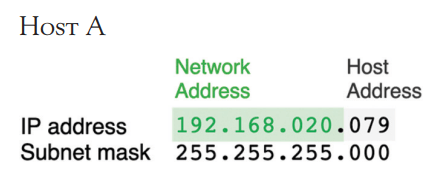
\includegraphics[width=67mm, keepaspectratio]{figures/host_a.png}
        \caption{Host A}
    \end{minipage}\hfill
    \begin{minipage}{0.45\textwidth}
        \centering
        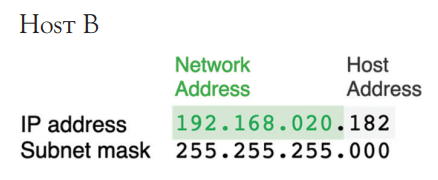
\includegraphics[width=67mm, keepaspectratio]{figures/host_b.png}
        \caption{Host B}
    \end{minipage}
\end{figure}
%----------------------------------------------------------------------------
Host A Host B  Host B ugyanabban az alhálózatban van,
mint Host A, mert mindkettő ugyanazt a hálózati címkét használja (192.168.020).
Az IP-cím hálózati része az a rész, ahol az alhálózati maszk 255-ös értéket
mutat. Ezen két eszköz között egy router sem szükséges. 
%----------------------------------------------------------------------------
\begin{figure}[H]
	\centering
	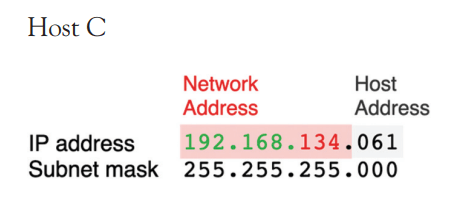
\includegraphics[width=67mm, keepaspectratio]{figures/host_c.png}
	\caption{Host C}
	\label {fig:host_c}
\end{figure}
%----------------------------------------------------------------------------
Host C más alhálózatban van, mint Host A és B, mert különbözik a hálózati címében (192.168.134, nem pedig 192.168.020).
Host C nem tud csomagokat cserélni A és B eszközökkel egy router nélkül. 
Annak érdekében, hogy ez az eszköz kommunikálhasson A és B-vel, más IP-címet kell kapnia,
kezdve a 192.168.134\ldots címmel. 
Vagy más alhálózati maszk is választható az egész beállításhoz,
például 255.255.0.0.
%----------------------------------------------------------------------------
A feljegyzett alhálózati maszkok decimális jelölése dot-decimális jelölésnek nevezik.
Azért, hogy az információt rövidebben jelezzék, gyakran
használt alternatív módszer a CIDR vagy perjeljelölés.
Az IP-cím után azonnal következő perjel után az
alhálózati maszkot a `0'-nál nagyobb értékeket mutatva jelöli meg.
Ez a jelölés az alhálózati maszk bináris formájára utal, tehát a `255' a `11111111' -nek felel meg.
A fenti példákban az alhálózati maszkok tehát bináris formájukban 24
`1'-t tartalmaznak. 
A fenti példában szereplő hosztok CIDR jelölése:
%----------------------------------------------------------------------------
\begin{itemize}
    \item \textbf{Host A:} 192.168.020.182/24
    \item \textbf{Host B:} 192.168.020.079/24
    \item \textbf{Host C:} 192.168.134.61/24
\end{itemize}
%----------------------------------------------------------------------------
A routereket használó és több alhálózatot összekapcsoló telepítések a
az OSI modell 3. rétegén működnek. Ez a modell hét rétegre osztja a
hálózatok általános funkcionalitását, mindegyik egy adott készletet ír le a hálózati
eszközök által nyújtott funkcionalitásokról. Gondolva itt elsősorban a csomagok továbbításáról a
megfelelő címzett felé. 

Az összes jelenlegi IT eszköz követi ezt a jól
meghatározott absztrakciós rétegkoncepciót, hogy elősegítse a gyártók közötti
interoperabilitást. A 3. rétegen működő telepítések értelmezhetik az IP-címeket,
az alhálózati maszkokat, és így továbbítani tudják a csomagokat az
alhálózatok között. Az itt tárgyalt összes technológia képes ilyen
forgatókönyvel működni. Ezzel szemben néhány technológia korlátozott a 2.
rétegre. Ez azt jelenti, hogy a csomagjaikat kizárólag MAC-címek alapján
szállítják, és nem tartalmaznak alhálózati információkat. Ennek eredményeként a
2. rétegű hálózatokat nem lehet több alhálózatokra bontani, a csomagjaikat nem
lehet routerek által továbbítani, és ezáltal a skálázhatóságuk korlátozott. 
Az egyik népszerű példa a 2. rétegű hálózatokra a már említett TSN/Milan, valamint a CobraNet.
%----------------------------------------------------------------------------
\begin{figure}[H]
	\centering
	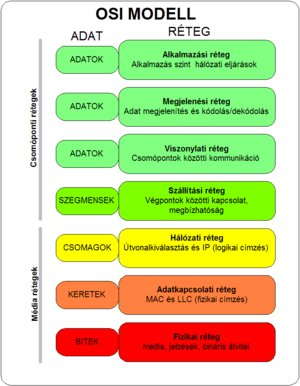
\includegraphics[width=100mm, keepaspectratio]{figures/osi_modell.jpg}
	\caption{Az OSI modell}
	\label {fig:osi_modell}
\end{figure}
%----------------------------------------------------------------------------
Egy alhálózat egy logikai szegmens egy adott hálózaton belül. Az ilyen szegmenseket
különféle okokból hoznak létre, ideértve elsősorban az adminisztratív és biztonsági
szempontokat. A hálózati adminisztrátor egy készlet szabályt alkalmazhat egy
alhálózatra, míg más szabályokat választhat egy másikra. A routerek képesek
összekapcsolni az alhálózatokat, így a hosztok csomagokat cserélhetnek az
alhálózati határok átlépése nélkül. Egy routernek megfelelően konfigurálva kell
lennie a hálózati útvonalak létrehozásához ezek között az alhálózatok között.
Ezzel szemben egy tipikus kapcsoló nem képes összekapcsolni az alhálózatokat.
Virtuális LAN készítése (VLAN) egy másik módszer a hálózat szegmentálására. 
Rugalmasabbá teszi a rendszereket, csökkenti a kapcsolatlan rendszerek közötti fölösleges kommunikációt.
Szemben az alhálózatokkal, ez egy biztonságosabb módja is a hosztok elkülönítésére egymástól.
%----------------------------------------------------------------------------
\subsection{Hálózati topológiák}
%----------------------------------------------------------------------------
A csomópontok különböző módon kapcsolódhatnak össze. A topológia meghatározása
az egyik legfontosabb döntés, amelyet egy hálózat tervezésekor hozni kell. A
csillag topológia sok szempontból preferált megoldás. Több hoszt egy
útválasztó eszközhöz, például egy kapcsolóhoz vagy routerhez csatlakozik. A mai
hálózatok gyakran két csillagszintet kombinálnak. Ezt gerinc/levél architektúrának
nevezik. A központi kapcsoló/router (gerinc) általában több forgalmat továbbít,
mint a perifériális kapcsoló (levél). Ha a gerinc és a levél közötti nagy sávszélességű
kapcsolat nem képes egyszerre továbbítani az összes hoszt forgalmát, akkor ez a
tervezési forma blokkoló. Az ellentéte egy nem blokkoló hálózattervezés, ahol a
nagy sávszélességű kapcsolatok képesek az összes a hozzájuk csatlakoztatott
hoszt teljes forgalmát folyamatosan továbbítani. 
A gyűrű topológiának több interfésze is lehet.
Legalább kettőre van szükség egy gyűrű topológia megvalósításához. Minden két
csomópont közötti kapcsolat teljes sávszélességet kínál, és a csomópontokra
hárul a feladat, hogy továbbítsák a csomagokat a gyűrűn belül. Ebben az
értelemben mindegyik csomópont úgy működik, mint egy kapcsoló, csomagokat
továbbítva két interfésze között. A gyűrű topológia választása gyakran ésszerű,
amikor nagy távolságokat kell áthidalni, és a kapcsolatok költségesek.
Gyakorlati példák a különböző helyszínek közötti hálózatok, de gyűrűket alkotnak
olyan eszközök csatlakoztatására is, amelyek esetében nincs hely egy további
kapcsoló számára. A gyűrű topológiák beépített redundanciát kínálnak minden
eszközhöz hozzáférhetünk, még akkor is, ha egy kapcsolat elszakad.
A megfelelő hálózat kialakításához még elengedhetetlenek a nem blokkoló kapcsolók.
A nem blokkoló architektúra egészében azt jelenti, hogy nem a kapcsolók a szűk keresztmetszet.
Tehát képesek kezelni az összes rájuk táplált forgalmat, csak a szabvány port sebessége a korlát.
%----------------------------------------------------------------------------
\subsection{Unicast és Multicast} %Egyedi és Csoportos Küldés
%----------------------------------------------------------------------------
Amikor egy eszköz csomagot küld egy másik eszköznek, ezt unicast mechanizmusnak
nevezzük. Egy ilyen kapcsolatnak pontosan egy küldője és egy fogadója van. Az
unicast használhatja a Transmission Control Protocol (TCP)-t, ahol a fogadó
minden egyes csomag sikerült átvételéről visszaigazolást küld a küldőnek. Ha a
visszaigazolás nem érkezik meg, a küldő automatikusan újraküldi a csomagot. 
Az UDP (User Datagram Protocol) egy alternatíva a TCP-nek. Ebben az esetben a küldő
bízik abban, hogy a csomagok sikeresen megérkeznek a fogadóhoz. Nincs
visszaigazolás, és ha a csomag elveszik, a tartalma is elveszik.
Ez az jelenti, hogy az UDP nem annyira megbízható? Valójában nem,
csak más felhasználásra hozták létre. 
Bár ez sokak számára váratlan lehet, valójában ez a preferált átviteli mód a szakmai audio hálózatok
számára. Mivel a késleltétésnek alacsonynak kell lennie, nem engedhető meg a
csomagok újraküldése, mert az értékes időt vesz igénybe, és ezzel növelné az általános
időkésleltetést. Az élő redszernél csomagvesztés esetén a legjobb, ha folytatjuk a
következő audio minták lejátszását, anélkül hogy megpróbálnánk helyreállítani az
előzőt. A menedzselhető switchek és végpontok tudják logolni a csomagvesztéseket, így
monitorozható a hálózat állapota amennyiben probléma merülne fel.
%----------------------------------------------------------------------------
\begin{figure}[H]
	\centering
	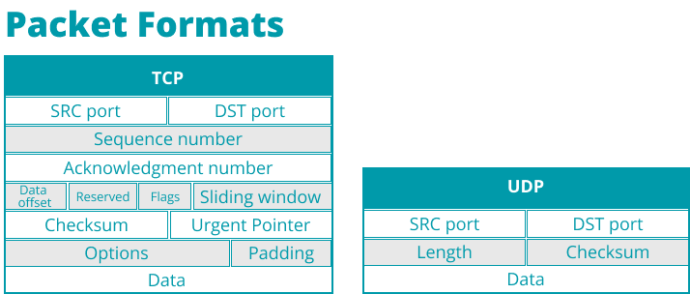
\includegraphics[width=100mm, keepaspectratio]{figures/tcp_udp.png}
	\caption{TCP és UDP összehasonlítás~\cite{TCPUDPPICS}}
	\label {fig:tcp_udp}
\end{figure}
%----------------------------------------------------------------------------
\begin{table}[h!]
	\centering
	\begin{tabular}{|l|p{5cm}|p{5cm}|}
	\hline
	\textbf{Jellemző} & \textbf{Transmission Control Protocol (TCP)} & \textbf{User Datagram Protocol (UDP)} \\
	\hline
	\textbf{Szolgáltatási típus} & Kapcsolatorientált protokoll; kapcsolat létesítése és lezárása szükséges az adatátvitel előtt és után. & Adatgramm-orientált protokoll; nincs szükség kapcsolat létesítésére vagy fenntartására, ideális broadcast és multicast esetén. \\
	\hline
	\textbf{Megbízhatóság} & Garantálja az adatok célba jutását. & Nem garantálja az adatok célba jutását. \\
	\hline
	\textbf{Hibajavító mechanizmus} & Kiterjedt hibajavító mechanizmusok, áramlás-ellenőrzés és adat-elismerés. & Alapvető hibajavító mechanizmus, ellenőrző összegeken alapul. \\
	\hline
	\textbf{Elismerés} & Van elismerési szegmens. & Nincs elismerési szegmens. \\
	\hline
	\textbf{Szekvenálás} & Garantálja a csomagok sorrendben érkezését. & Nincs adatcsomagok sorrendjének kezelése; ezt az alkalmazásrétegnek kell megoldania. \\
	\hline
	\textbf{Sebesség} & Lassabb, mint az UDP. & Gyorsabb, egyszerűbb és hatékonyabb. \\
	\hline
	\textbf{Csomagok újraküldése} & Lehetővé teszi az elveszett csomagok újraküldését. & Nincs újraküldés az elveszett csomagok esetén. \\
	\hline
	\textbf{Fejléc hossz} & 20-60 bájt között változhat. & Fix 8 bájt. \\
	\hline
	\textbf{Súly} & Nehéz súlyú. & Könnyű súlyú. \\
	\hline
	\textbf{Kézfogási technikák} & Kézfogások: SYN, ACK, SYN-ACK. & Kapcsolatmentes; nincs kézfogás. \\
	\hline
	\textbf{Broadcast támogatás} & Nem támogatja. & Támogatja. \\
	\hline
	\textbf{Protokollok} & HTTP, HTTPS, FTP, SMTP, Telnet. & DNS, DHCP, TFTP, SNMP, RIP, VoIP. \\
	\hline
	\textbf{Adatáram típus} & Bájtáram. & Üzenetáram. \\
	\hline
	\textbf{Túlterhelés} & Alacsony, de magasabb, mint az UDP. & Nagyon alacsony. \\
	\hline
	\textbf{Alkalmazások} & Biztonságos és megbízható kommunikáció, pl. e-mail, webes böngészés, katonai szolgáltatások. & Gyors kommunikáció, pl. VoIP, játékstreaming, video- és zene-streaming. \\
	\hline
	\end{tabular}
	\caption{A TCP és UDP összehasonlítása~\cite{UDP}}
	\label{tab:tcp_udp_comparison}
\end{table}
%----------------------------------------------------------------------------
Audio alkalmazásokban gyakran szükség van arra, hogy egy audio jelet
több helyre párhuzamosan fogadjanak, például egy mikrofonjel, amelyet
párhuzamosan továbbítanak a front-of-house és a monitoring keverőpultoknak. Akár
egy harmadik hely is létezhet, például egy felvevő eszköz. 
Amikor a küldő unicast módban továbbítja a csomagokat, az audio jel három csomagként
érkezik azonos tartalommal, de különböző címzettekkel. Ez felesleges
processzor terhelést jelent a küldő eszköz számára, és emellett külön sávszélességet is
foglal el mindhárom célhoz. Ezt lehet optimalizálni a multicast használatával. 
Számos előnye van, ideértve a küldőre nehezedő kevesebb processzor terhelést 
és az általános forgalom csökkenését a hálózaton. 
A küldő multicast címekre címezi a csomagokat, és nem hoszt címekre. Nem tudja, a csomagok címzettjeit. 
A multicast címek hasonlóak a rádiófrekvenciákhoz: bárki, aki érdeklődik, bekapcsolhatja és fogadhatja a
tartalmat. A küldő csak egyszer helyezi az audio adatokat egy csomagba, elküldi
egy multicast címre, és a vevőknek kell tudniuk, melyik multicast címre akarnak
hallgatni. A multicast címek alapvetően nem kapcsolódnak alhálózatokhoz, mivel nem
kapcsolódnak a csomópontokhoz és az IP-címekhez. Ezért a multicast csomagok
áthaladnak az alhálózatokon, hacsak nincsenek elkülönítve VLAN-okkal. 
Amennyiben a hálózatunk nem kizárólag az audio jelek továbbítására 
készült speciálisan, néhány eszköz lehet a hálózaton, amelyeknek semmi közük az audiohoz.
Ezért fontos, hogy a multicast forgalom csak
azokhoz a hosztokhoz jusson el, amelyek érdeklődnek iránta. 
Ennek a megoldása az IGMP snooping, tehát az Internet Csoportkezelési Protokoll. 
Az összes tárgyalt audio hálózati technológia alapértelmezetten
támogatja az IGMP snooping-ot. Ha be van kapcsolva a kapcsolóban, akkor a
multicast-csomagok csak azokon az interfészeken kerülnek elküldésre, ahol a
csatlakoztatott hosztoktól időszakos IGMP kérések érkeznek. Ha nincs beérkező
kérés, akkor a megfelelő multicast leáll, így nem jut felesleges forgalom a
kapcsolatra. Az IGMP snoopingot egyfajta zsilippel lehetne összehasonlítani,
amely alapértelmezetten zárva van, és csak kérésre nyílik meg. Erősen ajánlott
az IGMP snooping bekapcsolása egy multicast hálózatban minden egyes kapcsolóban.
Azonban egy hálózatban kizárólag csak egy darab IGMP Querier lehet aktív, mivel az
összes többi kapcsoló az aktív IGMP Querier-től kapja az információkat.
Enélkül a multicast úgy fog viselkedni mint egy broadcast, ami nagy mennyiségű
felesleges forgalmat eredményez, ezzel szennyezve a hálózatot.
Tehát a unicast a legjobb késleltetési teljesítményt nyújtja, és a
kapcsolók számára a legkönnyebben mozgatható.
A multicast pedig jobb sávszélesség-kezelést kínál, ahogy a csatornaszám és a sávszélességünk is nő.
%----------------------------------------------------------------------------
\subsection{Eszköz- és Adatfolyam-felfedezés}
%----------------------------------------------------------------------------
Az AES67 audió szabvány nem határozza meg, hogyan fedezhetik fel egymást a
hálózati eszközök, vagy hogy mely adatfolyamok érhetők el a hálózaton.
Az összes ismert technológia a bonjour vagy mDNS mechanizmust használja eszközeik számára
az egymásról való értesítésre. 
Minden eszköz fix és ismert multicast cím (224.0.0.251) felé küld
üzeneteket, amiket más eszközök is elérnek, így értesülnek egymás létezéséről a hálózatban.
Ennek a mechanizmusnak egyik korlátja az, hogy nem működik nagy telepítésekben,
ahol több alcímen vagy VLAN-on vannak különböző eszközök. Ezen esetekre a gyártók kifejlesztettek
saját megoldásokat (például Audinate a Dante Domain Manager-t) vagy
követik az audio/video NMOS szabványt a felismeréshez és kapcsolatkezeléshez.
Az audio adatfolyamokat a gyártótól függően két mechanizmus egyikével fedezik fel. Ahogy
az eszközök felfedezésénél, mindkettő előre meghatározott multicast címet
használ az adatfolyam-információk terjesztésére, hogy a címzettek megtalálják az
elérhető adatfolyamokat és azok paramétereit:
%----------------------------------------------------------------------------
\begin{itemize}
	\item Session Announcement Protocol (SAP) - minden Dante termék által használt (Multicast cím: 239.255.255.255)
\end{itemize}

\begin{itemize}
	\item Bonjour / mDNS - minden más technológiában használt (Multicast cím: 224.0.0.251) 
\end{itemize}
%----------------------------------------------------------------------------
Szerencsére a jelenlegi termékek többsége
lehetővé teszi mindkét protokoll egyidejű aktiválását, így egy adott audio
adatfolyam mindkét mechanizmuson keresztül párhuzamosan bejelenthető.
%----------------------------------------------------------------------------
\subsection{Redundancia}
%----------------------------------------------------------------------------
Az audiohálózatok kezdeti napjaiban egyes felhasználók kételkedtek az IT
hardverek megbízhatóságában. Annak ellenére, hogy ezek a széles körben elterjedt
IT-berendezések jól beváltak és gyakran megbízhatóbbnak viszonyulnak, mint a hagyományos
audioberendezések. Emellett a legtöbb hálózati komponens több diagnosztikai és monitorozási
mechanizmust kínál a berendezések hibájának gyors felismeréséhez és megoldásához.
%----------------------------------------------------------------------------
\subsubsection{Spanning Tree Protocol (STP)}
%----------------------------------------------------------------------------
Ha a kapcsolókat úgy kötik össze, hogy hurok jön létre, fennáll annak a veszélye, 
hogy a csomagok végtelenül áramlanak a hurokban. 
Ezt a \textit{visszacsatoló hurok} jelenséget a hálózati hardver automatikusan észleli az
STP segítségével, és ha hurokra bukkan, a kapcsoló automatikusan kikapcsolja egyik
kapcsolatot. Az STP-t továbbá felhasználhatják a rendszerben történő véletlen
kapcsolatvesztések elleni védelmére is, beleértve a kábelszakadásokat is. 

Ez abból a megközelítésből áll, hogy szándékosan létrehoznak hurkokat egyes végpontok között, majd a rendszer
inaktiválja az egyiket. Ha valamelyik kábel véletlenül kiesik, a rendszer
másodperceken belül észleli ezt, és újraaktiválja a passzív kapcsolatot. Ebben
az időszakban az audio néhány másodpercig ugyan megszakad, de még mindig sokkal
gyorsabb, mint a manuális hibakeresés és az új kábel telepítése, ha arra egyáltalán van lehetőségünk.
A legtöbb rendszerben az STP alapértelmezetten engedélyezve van. 
Nélküle broadcast 'viharok' alakulnának ki, ami konkrétan felemészti a sávszélességet.
%----------------------------------------------------------------------------
\subsubsection{Link Aggregáció}
%----------------------------------------------------------------------------
Ha egy adott kapcsolat különösen fontos egy telepítésben, két vagy több kábelt párhuzamosan
lehet csatlakoztatni a biztonság érdekében. 
Bár az ilyen link aggregáció fő célja két kapcsoló közötti sávszélesség növelése, 
ez is egy költséghatékony módszer lehet a kapcsolat véletlen leválasztásának
vagy kábelszakadás elleni védelmére. Tipikus eset például egy színpad, amely a FOH keverőhöz
csatlakozik. A kapcsolóknak mindkét végén ugyanúgy kell konfigurálni: két vagy
több interfészt kell kijelölni Link Aggregációs Csoportként, és azok
egyetlen interfészként jelennek meg a kapcsolón. Gyakorlatban a linkaggregáció
alkalmazása a kábelproblémák csökkentése érdekében nagyon hasznos lehet
egyszerűsége miatt, hiszen a felhasználónak csak egy további kábelt kell
biztosítania, és azonosítania kell a kapcsolók konfigurációját mindkét végén.
Ugyanakkor az éppen aktív kábel leválasztásakor előfordulhat, hogy az audioátvitel
néhány másodpercig itt is megszakad, mielőtt a kapcsoló az alternatív kapcsolatot
aktiválna.
%----------------------------------------------------------------------------
\subsubsection{ Adatfolyam redundancia}
%----------------------------------------------------------------------------
A legbiztonságosabb de egyben legdrágább módja a redundancia megvalósításának
egy hálózatban az, ha két különálló audiohálózatot hozunk létre, 
két független utat biztosítva a küldő és a fogadó között. 
Ebben a felállásban minden csomópontnak két hálózati interfészt
kell biztosítani. A küldő két azonos audio tartalommal rendelkező csomagot hoz létre,
mindkettőre azonos PTP-időbélyegzőt nyom, majd elküldi mindkét hálózaton.
A fogadó végén mindkét csomagot fogadják és kicsomagolják. Még akkor is, ha az egyik csomag
elveszik, a megmaradt csomag tartalmazza az összes információt, és biztosítja,
hogy az audio zavartalanul folytatódjon. Valójában ez a mechanizmus az egyetlen
megközelítés egy hálózatban a véletlenszerű csomagvesztés kompenzálására anélkül,
hogy meg kellene ismételni azokat a küldőtől és ezzel késleltetést hozzáadva a rendszerhez.
Ezzel a hangkimaradás problémáját is meg lehet oldani, mivel a redundáns csomagok
egyikének elvesztése esetén a másik csomagot használja a fogadó, így ez a procedúra
észrevehetetlen a felhasználó számára.
%----------------------------------------------------------------------------
\section{AES67~\cite{AHNERT2023}}
%----------------------------------------------------------------------------
Az AES67 szabvány szerint az összes eszköznek meg kell felelnie az
alábbi minimális specifikációknak: 
%----------------------------------------------------------------------------
\begin{itemize}
	\item Unicast és multicast támogatása
	\item UDP/RTP protokollok használata
	\item DSCP címkék beállítása meghatározott értékekre,QoS támogatás 
	\item Nincs meghatározott automatikus eszköz- és adatfolyam-felfedezés 
	\item PTPv2 szabvány használata az időszinkronizációhoz
	\item PTP profil Standard (a gyakorlatban a Dante jelenleg magasabb szinkronizációs rátát igényel)
	\item Küldőknek ki kell adniuk egy SDP fájlt
	\item A fogadóknak érteniük kell egy SDP fájlt
	\item A fogadó puffernek legalább 3 ms hangot kell tudnia tárolni
	\item Adatfolyam formátumok
	\item Egytől nyolc csatorna (a küldő választhat egy fix számot, de a fogadóknak képesnek kell lenniük rugalmasan fogadni bármelyik lehetőséget).
	\item 24 bites és 16 bites felbontás (a küldő választhat egyet, de a fogadóknak mindkettőt érteniük kell) 
	\item 48 kHz mintavételi frekvencia 1 ms csomagidő (48 minta)
	\item A multicast címek 239.0.0.0 és 239.255.255.255 között vannak 
\end{itemize}
%----------------------------------------------------------------------------
A szabványban sok további paraméter és érték szerepel, de ezek nem szerepelnek a
fent felsorolt minimális követelmények között.
%----------------------------------------------------------------------------
\section{Audinate Dante~\cite{AHNERT2023}}
%----------------------------------------------------------------------------
\subsection{A cégről~\cite{AUDINATEHISTORY}} %https://www.audinate.com/company/history
%----------------------------------------------------------------------------
Az Audinate a professzionális AV hálózati technológiák vezető globális szolgáltatója, 
az AV és IT rendszerek konvergenciájában játszik kulcsszerepet Dante platformjával. 

Az Audinate gyökerei Sydney-ben találhatók, ahol egy kis mérnökcsapat a Motorola 
Kutatólaboratóriumában fejlesztett új technológiákat. A Motorola 2003-ban bezárta 
a létesítményt, de néhány mérnök tovább dolgozott a Nemzeti Információs és 
Kommunikációs Technológiai Intézettel (NICTA), egy ausztrál kormányzati kutatóintézettel 
karöltve, amely az ipari növekedést elősegítő innovatív technológiák fejlesztését támogatta. 
A cég irányvonalát Aidan Williams, társalapító és technológiai igazgató érdeklődése 
a zene iránt határozta meg, míg IT-szakértői szemlélete kijelölte a technológiai utat.

2006-ban a NICTA felismerte a technológia potenciálját, és az Audinate kivált az 
intézményből, hogy kereskedelmi forgalomba hozza Dante hálózati technológiáját. 
A csapat 2008-ban talált rá egy korai támogatóra Bruce Jackson személyében, aki 
a Dolby Labs élő hangosztályának alelnöke volt. A Dante technológia gyorsan 
elterjedt a professzionális audioiparban, számos jelentős eseményen és helyszínen, 
köztük az olimpiai játékokon és nagy zenei koncerteken alkalmazták.
%----------------------------------------------------------------------------
\begin{figure}[H]
	\centering
	
\includegraphics[width=50mm, keepaspectratio]{figures/audinate_logo.png}
	\caption{Az Audinate logója}
	\label {fig:audinate_logo}
\end{figure}
%----------------------------------------------------------------------------
2014-re már több mint 170 gyártó használta a Dante technológiát, és a termékek 
száma meghaladta a 675-öt. 2016-ra az Audinate új termékeket mutatott be, például 
a Dante Analog Output Module-t, amely lehetővé tette az analóg eszközök 
csatlakoztatását a Dante hálózathoz. 2017-ben a Dante Domain Manager és a 
Dante Broadway is piacra került, melyek tovább bővítették a technológia alkalmazási lehetőségeit.

Az évek során az Audinate folyamatosan növekedett és új termékekkel jelentkezett, 
mint például a Dante AVIO adapterek 2018-ban, valamint a Dante AV technológia 2019-ben, 
amely integrálta az audio- és videojelek hálózaton keresztüli továbbítását. 2020-ban, 
a globális járvány idején, a Dante AV termékek új lehetőségeket nyitottak meg az 
otthoni munkavégzés és biztonságos konferenciatermi megoldások számára.

2024-re az Audinate több mint 600 gyártóval kötött licencszerződést, és a Dante 
technológiát több mint 4000 termékben használják, beleértve az AV és IT rendszerek 
teljes integrálását és kezelését, világszerte.
%----------------------------------------------------------------------------
\subsection{A Dante hálózatok áttekintése}
%----------------------------------------------------------------------------
A 2020-2021-es Covid-19 járvány során lehetőségem volt részt venni egy átfogó Dante
kurzuson, amelyet a Dante technológia fejlesztője, az Audinate szervezett. A kurzus
részletes betekintést nyújtott a Dante hálózatok működésébe. E fejezetben a belsős
oktatóanyagokat is fel fogom felhasználni, amelyeket a kurzus alatt kaptam. Ezek a dokumentumok
csak a kurzus résztvevői számára elérhetők, így konkrét dokumentumként nem publikálhatók. 
%Ebből következően ezen írásokat konkrét hivatkozások nélkül fogom felhasználni, mivel
%hivatkozásuk nem lehetséges.
%Viszont fontos megjegyezni, hogy a fejezetben szereplő ábrák és információk az Audinate tulajdonát képezik.

A Dante hálózatok a digitális hangátviteli technológia egy korszerű formáját képviselik, 
amely lehetővé teszi a hang elosztását és irányítását szabványos Ethernet alapú hálózatokon 
keresztül. Az ausztrál Audinate által kifejlesztett Dante technológia IP hálózatokat használ 
a magas minőségű, alacsony késleltetésű hangátvitel biztosítására az eszközök között. 

Ez a rendszer jelentős előnyöket nyújt a hagyományos analóg hangrendszerekhez képest, 
beleértve a nagyobb rugalmasságot és skálázhatóságot, valamint lehetőséget ad a hangrendszerek 
integrálására meglévő IT infrastruktúrákba. 

A Dante technológia széles körben elterjedt, többek között a koncerthangosítás, rádiózás, 
stúdiófelvételek, vállalati környezetek és konferenciaközpontok területén. Támogatja a különböző 
hangformátumokat és mintavételi rátákat, és lehetővé teszi akár több száz hangcsatorna egyidejű 
átvitelét egyetlen hálózaton keresztül. Továbbá, a Dante rendszerek távolról vezérelhetők és 
monitorozhatók, ami jelentősen megkönnyíti a komplex hangrendszerek beállítását és kezelését.
%----------------------------------------------------------------------------
\subsection{Dante hálózatok technikai részletei}
%----------------------------------------------------------------------------
A Dante hanghálózatok két alapvető elemből épülnek fel: a Dante eszközökből és a Dante hálózatokból. 
A Dante eszközök speciálisan a Dante protokollhoz készült hangeszközök, mint például hangkártyák, erősítők és hangládák. 
Ezek az eszközök szabványos Ethernet kábeleken és kapcsolókon keresztül csatlakoznak a Dante hálózathoz. 

A hálózat konfigurálása az Audinate Dante Controller szoftver segítségével történik, amely lehetővé teszi a hang elosztását és 
irányítását az eszközök között. A szoftver lehetőséget ad az eszközök távoli vezérlésére és monitorozására. 
A Dante hanghálózatok különböző hangformátumokat és mintavételi rátákat támogatnak, és képesek egyszerre több száz hangcsatorna 
átvitelére egyetlen hálózaton keresztül. Továbbá, a technológia fejlett funkciókat is biztosít, mint a Dante Domain Manager (DDM), 
amely a biztonságos hangátvitelt szolgálja, és a Dante Virtual Soundcard (DVS), amely számítógépes hanglejátszást és felvételt 
lehetővé téve.

Amennyiben több eszköz hangot küld egy adott végpontra a hálózaton, az alapértelmezett működés szerint a csomagok felgyülemlése 
esetén az elsőként érkezők előnyben részesülnek. A Dante hanghálózatok Quality of Service (QoS) támogatást is nyújtanak, 
amely a prioritások kezelését biztosítja. Ezáltal a hangátvitel előnyt élvezhet más hálózati forgalommal szemben, csökkentve 
a hálózati torlódás esélyét és biztosítva a minimális késleltetést valamint a magas minőséget. Körülbelül 70 százalékos 
hálózati szaturációnál már javasolt a QoS alkalmazása, míg 100 Mbps sebességű hálózatok esetén a jitter csökkentésére is 
segít.
%----------------------------------------------------------------------------
\subsubsection{Több mintavételi ráta és bitmélység}
%----------------------------------------------------------------------------
A rendszer képes egyidejűleg több bitmélységet kezelni. Ennek informatikai háttere a
a következő képpen néz ki:
Ha egy 32 bites hangforrásunk van, de a másik eszköz
csak 24 bites hangot tud fogadni, akkor a Dante a 32 bites hangot 24 bitesre tudja 
alakítani.
%----------------------------------------------------------------------------
\begin{table}[h!]
	\centering
	\begin{tabular}{|c|c|}
	\hline
	\textbf{Hangminták} & \textbf{Bitmélység} \\
	\hline
	\texttt{11110000 11110000 11110000 11110000} & 32 bites \\
	\hline
	\texttt{11110000 11110000 11110000} & 24 bites \\
	\hline
	\end{tabular}
	\caption{32 bites és 24 bites hangminták}
	\label{tab:bit_depth_example}
\end{table}
%----------------------------------------------------------------------------
Amint a példában látszik, 32 bites hangból úgy kaptunk 24 bites hangot, 
hogy egyszerűen csak elhagytuk az utolsó 8 bitet. Ez a folyamat visszafelé is működik,
ha 24 bites hangot kell 32 bites hanggá alakítani, akkor az utolsó 8 bitet 0-val kell feltölteni.
%----------------------------------------------------------------------------	
\begin{table}[h!]
	\centering
	\begin{tabular}{|c|c|}
	\hline
	\textbf{Hangminták} & \textbf{Bitmélység} \\
	\hline
	\texttt{11110000 11110000 11110000} & 24 bites \\
	\hline
	\texttt{11110000 11110000 11110000 00000000} & 32 bites \\
	\hline
	\end{tabular}
	\caption{24 bites hangból 32 bites hang}
	\label{tab:bit_depth_conversion}
\end{table}
%----------------------------------------------------------------------------
A mintavételezési frekvencia eltérése csak akkor kezelhető, ha a bitmélység is különbözik. 
Amennyiben a bitmélység megegyezik, de a mintavételezési frekvencia eltér, a rendszer nem 
képes a hang megfelelő továbbítására. Ez a mechanizmus egy egyszerű mechanikai példával 
érthető és szemléltethető. Képzeljünk el két fogaskereket: ha a mintavételezési frekvencia 
azonos, de a bitmélység eltérő, akkor a fogaskerekek egymásba illeszthetőek, és csupán a 
fogaskerekek mélysége fog eltérni. Viszont, ha a mintavételezési frekvencia eltérő, a 
fogaskerekek nem illeszthetőek egymásba, így a hang továbbítása lehetetlenné válik. 
Ebben az esetben szükség van egy konverterre, amely képes a két fogaskereket összeilleszteni. 
Fontos megjegyezni, hogy a több mintavételi ráta együttes működése érdekében egységes 
órajel szükséges minden mintavételi frekvenciához.
%----------------------------------------------------------------------------
\subsubsection{Hálózati topológiák}
%----------------------------------------------------------------------------
A Dante rendszerek alapvetően két üzemmódban működhetnek. Az egyik az ún. 
switched (kapcsolt) mód, ahol az eszközökön található két Ethernet port egyetlen 
hálózatot alkot. Ebben a módban lehetőséget biztosítunk Daisy Chain (füzéres) 
topológia kialakítására, ahol az egyik eszköz a következőhöz csatlakozik, és így tovább. 
Emellett csillagtopológia is létrehozható, ahol minden eszköz egy központi kapcsolóhoz 
csatlakozik.
%----------------------------------------------------------------------------
\begin{figure}[H]
	\begin{minipage}{0.5\textwidth}
		\centering
		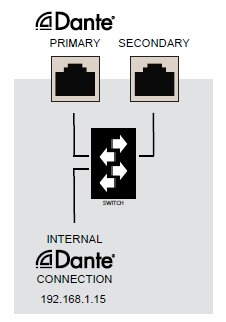
\includegraphics[width=100px, keepaspectratio]{figures/dante-switched-mode.jpg}
		\caption{Kapcsolt mód}
		\label{fig:dante_switched}
	\end{minipage}%
	\begin{minipage}{0.5\textwidth}
		\centering
		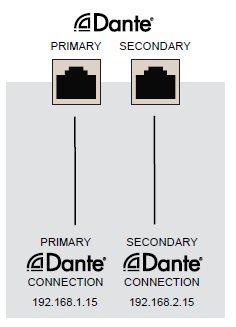
\includegraphics[width=100px, keepaspectratio]{figures/dante-redundant-mode.jpg}
		\caption{Redundáns mód}
		\label{fig:dante_redundant}
	\end{minipage}
\end{figure}
%----------------------------------------------------------------------------
A másik üzemmód a redundant (redundáns) üzemmód, amelyben az eszközök két 
Ethernet portja két különálló hálózatot alkot. Ez a konfiguráció biztosítja, hogy 
a hálózat redundáns módon van kialakítva, így ha az egyik rész meghibásodik, 
a másik automatikusan átvállalja annak szerepét. 
Bizonyos Dante eszközök rendelkeznek egy harmadik Ethernet porttal, 
amelyet konfigurálási és vezérlési feladatokra használnak.
%----------------------------------------------------------------------------
\subsubsection{Késleltetés}
%----------------------------------------------------------------------------
A késleltetés az az időtartam, amely szükséges egy folyamat végrehajtásához, 
például a bemeneti oldalon beérkező hangjel feldolgozásához és annak megjelenéséhez 
a kimeneti oldalon. A késleltetés mérésére két fő mértékegységet használunk:
%----------------------------------------------------------------------------
\begin{align}
    1 \text{ másodperc} &= 1000 \text{ milli másodperc}, \quad \text{azaz} \quad 1 \text{ ms} = 0.001 \text{ s} \\
    1 \text{ másodperc} &= 1000000 \text{ mikro másodperc}, \quad \text{azaz} \quad 1 \mu\text{s} = 0.000001 \text{ s}
    \label{eq:microseconds}
\end{align}
%----------------------------------------------------------------------------
A Dante eszközök lehetőséget biztosítanak a késleltetés teljesítményének 
meghatározására. A 0.1 milliszekundumos késleltetés az, amely már biztosítja a 
kapcsoló lépést. Ha két eszköz késleltetése eltérő, akkor a nagyobb érték számít 
irányadónak. Egy megfelelően beállított modern Dante hálózatban a késleltetés 
körülbelül 1 ms értéket vesz fel, ami azt jelenti, hogy például egy dobos 
először hallja a hangszerét a fülmonitoron, mint a saját dobját.
%----------------------------------------------------------------------------
\subsubsection{Órajel}
%----------------------------------------------------------------------------
Minden eszköz egy rendkívül pontos Dátum/Idő órát követ, amely biztosítja az 
idő szinkronizációját és az egységes sebességet. De mi a helyzet a terjedési 
késéssel? Miért vannak szinkronban a Dante eszközök? A PTP (Precision Time Protocol) 
késleltetési kéréseket (Delay Requests) indít, amelyek segítségével kiszámítják 
a hálózat késleltetését. Az eszközök az információátvitel késését is kompenzálják. 
A Dante automatikusan kiválaszt egy óra vezetőt, és mindig csak egyetlen óra 
vezető létezik, függetlenül a mintavételi rátától. Szükség esetén külső óra 
vezetőt is beállíthatunk. A rendszer nem szinkronizál újra, hanem beállítja 
a sebességet és kompenzálja a hálózati késést. A Dante által végzett tesztelések 
és tapasztalatok alapján igazolt, hogy az időzítés szinkronban marad, még akkor 
is, ha az óra perceken keresztül teljesen eltűnik.
%----------------------------------------------------------------------------
\begin{figure}[H]
	\centering
	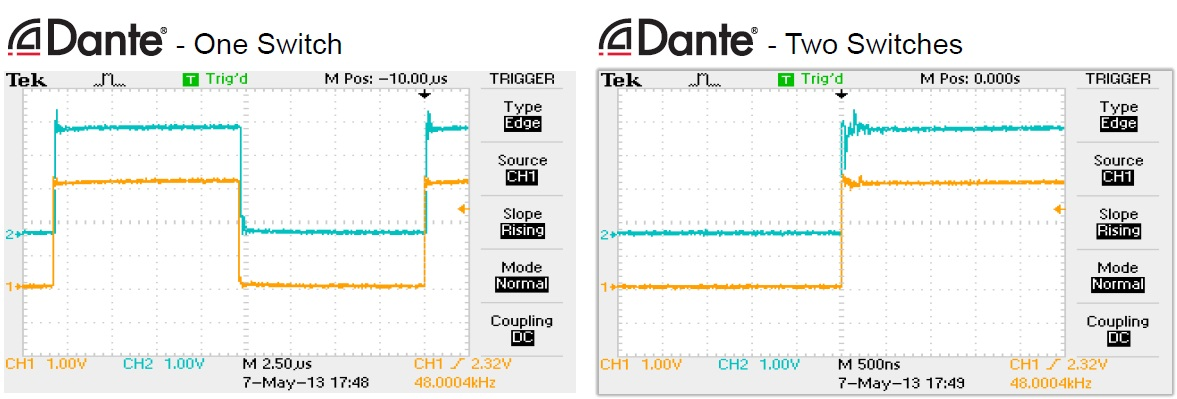
\includegraphics[width=400px, keepaspectratio] {figures/dante-clocking.jpg}
	\caption{Dante órajel}
	\label{fig:dante-clock}
\end{figure}
%----------------------------------------------------------------------------
\subsection{Összehasonlítás a hagyományos hangrendszerekkel}
%----------------------------------------------------------------------------
A hagyományos hangrendszerek általában analóg kábeleken és csatlakozókon alapulnak 
a hangjelek eszközök közötti továbbítására. E rendszerek gyakran korlátozottak 
a rugalmasság, a skálázhatóság, valamint az egyidejűleg kezelhető hangcsatornák 
számát tekintve. Továbbá, a beállításuk és kezelési folyamatuk bonyolultabb lehet, 
mivel minden egyes hangcsatorna külön kábel és csatlakozás igényel. Ezzel szemben 
a Dante hanghálózatok jelentős előnyöket kínálnak: lényegesen több hangcsatorna 
támogatására képesek, lehetővé téve a nagy és összetett hangrendszerek egyszerű 
beállítását és kezelését. A Dante rendszer emellett képes hosszú távolságokon 
továbbítani a hangot anélkül, hogy a minőség romlana. Ezzel szemben a hagyományos 
analóg rendszerek hosszú kábelek használata során hajlamosak zajra és jelveszteségre, 
míg a digitális hangjelek, amelyeket Ethernet hálózatokon továbbítanak, minimális 
minőségveszteséggel érhetők el nagy távolságokra.
%----------------------------------------------------------------------------
\begin{table}[htbp]
    \centering
    \caption{Digital Snake és DigitalAVNetwork Jelút opciók}
    \begin{tabular}{@{}lll@{}}
        \toprule
        \textbf{Kérdés} & \textbf{Pont-pont között} & \textbf{Hálózati megoldás} \\ \midrule
        Hová megy a jel? & Lineáris kábelút & Bárhol a hálózaton \\
        Hogyan változtassuk meg a jelútvonalat? & Mozgassuk a kábelt & Egy egérkattintással \\
        Szétválaszthatjuk-e a jeleket? & Nem & Igen - a hálózaton \\
        Megosztható-e a kábel más jelekkel? & Nem & Igen - közös infrastruktúra \\
        \bottomrule
    \end{tabular}
    \label{tab:digital-snake-vs-digitalavnetwork-hu}
\end{table}
%----------------------------------------------------------------------------
\begin{figure}[H]
	\centering
	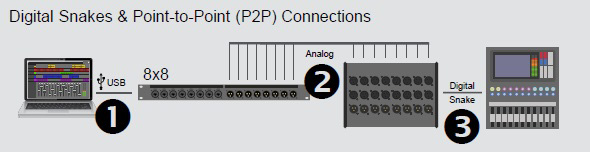
\includegraphics[width=\linewidth, keepaspectratio]{figures/dsnake-p2p.jpg}
	\caption{Digital Snake és Pont-pont közötti (P2P) kapcsolatok}
	\label {fig:dsnake-p2p}
\end{figure}
%----------------------------------------------------------------------------
\begin{figure}[H]
	\centering
	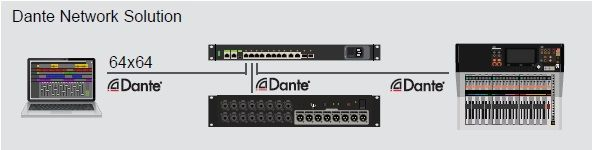
\includegraphics[width=\linewidth, keepaspectratio]{figures/dante-solution.jpg}
	\caption{Dante hálózati megoldás}
	\label {fig:dante-solution}
\end{figure}
%----------------------------------------------------------------------------
A rugalmasság és a skálázhatóság tovbbi kulcsfontosságú előnye a Dante
hanghálózatoknak a hagyományos analóg hangrendszerekkel szemben.
Képesek alkalmazkodni különböző hangkonfigurációkhoz és követelményekhez. 
Könnyű eszközöket hozzáadni vagy eltávolítani, megváltoztatni a hangjelek útvonalát, és a rendszert újra
konfigurálni szükség esetén. Ez lehetővé teszi testreszabott audio-megoldások
létrehozását, amelyeket az adott alkalmazás vagy környezet speciális igényeihez
lehet igazítani. 
%----------------------------------------------------------------------------
\subsection{Firmware frissítés}
%----------------------------------------------------------------------------
A Dante eszközök két típusú firmware-rel rendelkeznek: a Dante Firmware-rel és az 
Eszköz Firmware-rel. A rendszer megfelelő működése érdekében előfordulhat, hogy mindkét 
firmware-t frissíteni kell. A frissítések összehangolt verziói biztosítják a legjobb 
kompatibilitást és működést. A szükséges verziók pontos meghatározásához a gyártóval 
való konzultáció ajánlott.

Az eszközkategóriák között különbségek lehetnek a frissítési eljárásokban. Bizonyos 
eszközök esetén alternatív frissítési módszerek állnak rendelkezésre, míg a Dante 
Updater szoftver egy széles körben alkalmazott eszköz, amely segíti a frissítési 
folyamatok egyszerűsítését. A Dante Updater rendszeresen ellenőrzi az online 
adatbázisokat, és értesít a legfrissebb firmware verziókról.

A firmware frissítési folyamat megkönnyítése érdekében ajánlott a Dante Firmware 
Update Manager használata, amely lehetővé teszi a frissítési fájlok importálását, 
például ha a gyártó közvetlenül biztosít firmware fájlokat. Sikertelen frissítés 
esetén vészhelyzeti helyreállítási eljárások állnak rendelkezésre, amelyek biztosítják 
az eszköz biztonságos helyreállítását.

A Dante eszközök támogatják a vegyes firmware verziókat, lehetővé téve az eltérő 
verziók együttműködését. Ezt a funkciót rendszeres automatizált regressziós tesztelés 
biztosítja, amely a különböző firmware verziók közötti kompatibilitást ellenőrzi.
%----------------------------------------------------------------------------
\subsection{Chipek}
%----------------------------------------------------------------------------
A Dante hálózatok különféle chipekkel építhetők fel. Az Audinate széles választékot 
kínál a Dante rendszerhez tervezett chipekből, amelyek eltérő hangcsatorna-számot 
és további funkciókat támogatnak. A Dante chipek különböző méretekben és árkategóriákban 
érhetők el, lehetővé téve a gyártók számára, hogy különböző méretű és költségű Dante 
eszközöket fejlesszenek ki, így kielégítve a változatos piaci igényeket. A Dante chipek 
elősegítik a gyártók munkáját azáltal, hogy lehetővé teszik a Dante-kompatibilis eszközök 
gyors és hatékony létrehozását, valamint egyszerű integrációjukat a meglévő termékekbe.
%----------------------------------------------------------------------------
\begin{table}[h!]
	\centering
	\begin{tabular}{|c|p{10cm}|}
		\hline
		\textbf{Chip} & \textbf{Leírás} \\
		\hline
		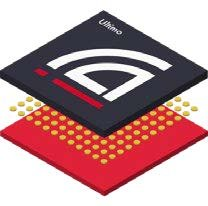
\includegraphics[width=40px,height=40px,keepaspectratio]{figures/ultimo-x.jpg} & \textbf{Dante Ultimo-X} - 0x4, 2x2, 4x0 \\
		\hline
		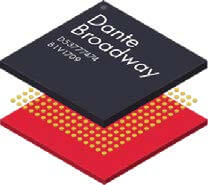
\includegraphics[width=40px,height=40px,keepaspectratio]{figures/broadway.jpg} & \textbf{Dante Broadway} - 16x16 \\
		\hline
		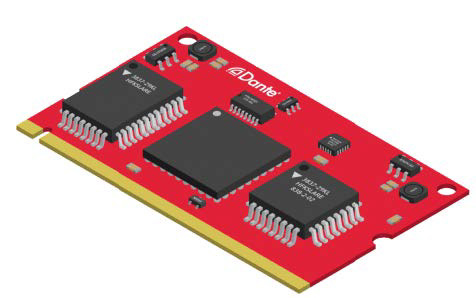
\includegraphics[width=40px,height=40px,keepaspectratio]{figures/brooklyn-ii.jpg} & \textbf{Dante Brooklyn II} - 64x64 \\
		\hline
		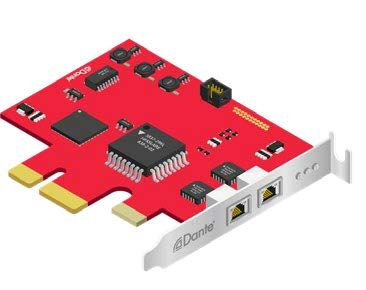
\includegraphics[width=40px,height=40px,keepaspectratio]{figures/pcie-r.jpg} & \textbf{Dante PCIe-R} - 128x128 \\
		\hline
		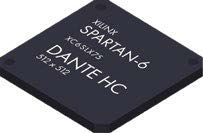
\includegraphics[width=40px,height=40px,keepaspectratio]{figures/dante-hc.jpg} & \textbf{Dante HC (High Capacity)} - 512x512 \\
		\hline
		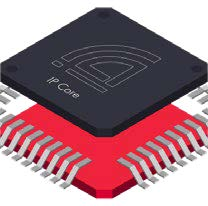
\includegraphics[width=40px,height=40px,keepaspectratio]{figures/shared-processor.jpg} & \textbf{Dante Shared Processor} - IP Core 512x512 FPGA and Dante Embedded Platform 64x64 X86/ARM \\
		\hline
		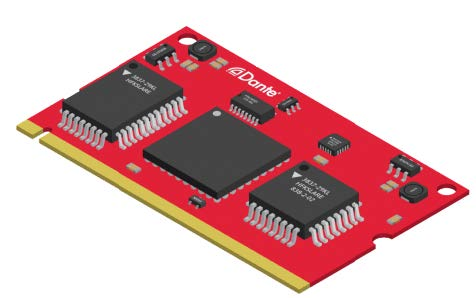
\includegraphics[width=40px,height=40px,keepaspectratio]{figures/dante-av.jpg} & \textbf{Dante AV} - V:1, A:8 \\
		\hline
	\end{tabular}
	\caption{Különböző Dante chipek}
	\label{tab:dante_chips}
\end{table}
%----------------------------------------------------------------------------